% vi:tw=80:
\documentclass[dvipsnames,a0paper,portrait]{baposter}
%\documentclass[portrait,final]{baposter}
%\documentclass[a4shrink,portrait,final]{baposter}
% Usa a4shrink for an a4 sized paper.

\tracingstats=2

%\usepackage{times}
\usepackage{calc}
\usepackage{graphicx}

\usepackage{amsmath}
\usepackage{amssymb}
\usepackage{relsize}
\usepackage{multirow}
\usepackage{bm}
\usepackage[UKenglish]{babel}
\usepackage{paralist}
\usepackage{booktabs}
\usepackage{subfig}
\usepackage{url}
\hyphenation{except}

\pdfpageattr {/Group << /S /Transparency /I true /CS /DeviceRGB>>}

\usepackage{adjustbox}
\usepackage{pgfplots}
\pgfplotsset{width=0.5\columnwidth,compat=1.10}

\usepackage{graphicx}
\usepackage{multicol}

\usepackage{pgfbaselayers}
\pgfdeclarelayer{background}
\pgfdeclarelayer{foreground}
\pgfsetlayers{background,main,foreground}

\usepackage{helvet}
\usepackage[utf8]{inputenc}
\usepackage[T1]{fontenc}
%\usepackage{berling}
%\usepackage{gillaltmt}
\usepackage{palatino}

%\newcommand{\captionfont}{\footnotesize}

\newcommand\chunk[2]{\ensuremath{\mbox{[#2]}_{\mbox{\tiny#1}}}}

\selectcolormodel{cmyk}

%\graphicspath{{images/}}

%%%%%%%%%%%%%%%%%%%%%%%%%%%%%%%%%%%%%%%%%%%%%%%%%%%%%%%%%%%%%%%%%%%%%%%%%%%%%%%%
% Multicol Settings
%%%%%%%%%%%%%%%%%%%%%%%%%%%%%%%%%%%%%%%%%%%%%%%%%%%%%%%%%%%%%%%%%%%%%%%%%%%%%%%%
\setlength{\columnsep}{0.7em}
\setlength{\columnseprule}{0mm}


%%%%%%%%%%%%%%%%%%%%%%%%%%%%%%%%%%%%%%%%%%%%%%%%%%%%%%%%%%%%%%%%%%%%%%%%%%%%%%%%
% Save space in lists. Use this after the opening of the list
%%%%%%%%%%%%%%%%%%%%%%%%%%%%%%%%%%%%%%%%%%%%%%%%%%%%%%%%%%%%%%%%%%%%%%%%%%%%%%%%
%\newcommand{\compresslist}{%
%\setlength{\itemsep}{1pt}%
%\setlength{\parskip}{0pt}%
%\setlength{\parsep}{0pt}%
%\setlength{\leftmargin}{10cm}%
%}
\setdefaultleftmargin{1em}{}{}{}{.5em}{.5em}

%%%%%%%%%%%%%%%%%%%%%%%%%%%%%%%%%%%%%%%%%%%%%%%%%%%%%%%%%%%%%%%%%%%%%%%%%%%%%%
%%% Begin of Document
%%%%%%%%%%%%%%%%%%%%%%%%%%%%%%%%%%%%%%%%%%%%%%%%%%%%%%%%%%%%%%%%%%%%%%%%%%%%%%

\begin{document}

%%%%%%%%%%%%%%%%%%%%%%%%%%%%%%%%%%%%%%%%%%%%%%%%%%%%%%%%%%%%%%%%%%%%%%%%%%%%%%
%%% Here starts the poster
%%%---------------------------------------------------------------------------
%%% Format it to your taste with the options
%%%%%%%%%%%%%%%%%%%%%%%%%%%%%%%%%%%%%%%%%%%%%%%%%%%%%%%%%%%%%%%%%%%%%%%%%%%%%%
% Define some colors
\definecolor{uured}{RGB/cmyk}{153,0,0/0,.91,.72,.23}
\definecolor{emphgreen}{RGB}{0,210,0}

\definecolor{silver}{cmyk}{0,0,0,0.3}
\definecolor{yellow}{cmyk}{0,0,0.9,0.0}
\definecolor{reddishyellow}{cmyk}{0,0.22,1.0,0.0}
\definecolor{black}{cmyk}{0,0,0.0,1.0}
\definecolor{darkYellow}{cmyk}{0,0,1.0,0.5}
\definecolor{darkSilver}{cmyk}{0,0,0,0.1}

\definecolor{lightyellow}{cmyk}{0,0,0.3,0.0}
\definecolor{lighteryellow}{cmyk}{0,0,0.1,0.0}
\definecolor{lighteryellow}{cmyk}{0,0,0.1,0.0}
\definecolor{lightestyellow}{cmyk}{0,0,0.05,0.0}

\newcommand\alert{\textcolor{uured}}
\newcommand\green{\textcolor{emphgreen}}

%\newcommand\redbox[1]{\fcolorbox{uured}{white}{%
%        \parbox{\textwidth - 2\fboxsep}{#1}}}
\newsavebox{\tmpredbox}
\newcommand\redbox[1]{%
\savebox{\tmpredbox}{%
\begin{minipage}{\textwidth-2\fboxsep}%
#1%
\end{minipage}}%
\tikz \draw(0,0) node[style=draw,inner sep=1.2\fboxsep,color=uured]%
      {\usebox{\tmpredbox}};}

\newcommand\figredbox[1]{%
\savebox{\tmpredbox}{%
\begin{minipage}{\textwidth-2\fboxsep}%
#1%
\end{minipage}}%
\tikz \draw(0,0) node[style=draw,color=uured]%
      {\usebox{\tmpredbox}};}
\newcommand\sect[1]{\alert{\textbf{\large #1}}\par}

%%
\typeout{Poster Starts xxx}
\background{
  \begin{tikzpicture}[remember picture,overlay]%
    \draw (current page.south east)+(1.5em,0em)
       node[opacity=0.1,anchor=south east]
       {\includegraphics[height=.8\textheight]{18370_UU_sigill_NV}};
    \draw (current page.north west) node[anchor=north west]
       {\includegraphics[height=42mm]{UU_logo_4f_42}};
    \draw[uured] ($(current page.north west)+(0mm,-42mm)$)
       -- ($(current page.north east)+(0mm,-42mm)$);
  \end{tikzpicture}%
}



\newlength{\leftimgwidth}
\begin{poster}%
  % Poster Options
  {
  % Show grid to help with alignment
  grid=false,
  columns=2,
  % Column spacing
  colspacing=1.5em,
  % Color style
  %bgColorOne=lighteryellow,
  %bgColorTwo=lightestyellow,
  %borderColor=reddishyellow,
  %headerColorOne=yellow,
  %headerColorTwo=reddishyellow,
  %headerFontColor=black,
  %boxColorOne=lightyellow,
  %boxColorTwo=lighteryellow,
  bgColorOne=white,
  bgColorTwo=white,
  borderColor=uured,
  headerColorOne=uured,
  headerColorTwo=reddishyellow,
  headerFontColor=white,
  boxColorOne=white,
  boxColorTwo=white,
  % Format of textbox
  %textborder=coils,
  % Format of text header
  %eyecatcher=yes,
  headerborder=open,
  headerheight=0.12\textheight,
  headershape=rectangle,
  headershade=plain,
  %headerfont=\Large\textsf, %Sans Serif
  headerfont=\Large\textbf,
  textborder=none,
  boxshade=none,
  background=user,
%  background=plain,
  linewidth=2pt
  }
  % Eye Catcher
  {}
  % Title
  {
  \hspace*{.17\textwidth}%
  \parbox{.83\textwidth}{%
    \normalfont
    {\sffamily POS Driven Cross-Lingual Pronoun Prediction \\ with Feed-Forward Neural Networks\\
    {\Large Jimmy Callin, Christian Hardmeier, Jörg Tiedemann}}}}
  % Authors
  {}
  % University logo
  {
    % The makebox allows the title to flow into the logo, this is a hack because of the L shaped logo.
    %\makebox[8em][r]{%
      %\begin{minipage}{16em}
        %\hfill
        %\includegraphics[height=2em]{msrlogo}
        %\includegraphics[height=7.0em]{logo}
      %\end{minipage}
    %}
  }

  \tikzstyle{light shaded}=[top color=baposterBGtwo!30!white,bottom color=baposterBGone!30!white,shading=axis,shading angle=30]

  % Width of left inset image
     \setlength{\leftimgwidth}{0.78em+8.0em}

%%%%%%%%%%%%%%%%%%%%%%%%%%%%%%%%%%%%%%%%%%%%%%%%%%%%%%%%%%%%%%%%%%%%%%%%%%%%%%
%%% Now define the boxes that make up the poster
%%%---------------------------------------------------------------------------
%%% Each box has a name and can be placed absolutely or relatively.
%%% The only inconvenience is that you can only specify a relative position
%%% towards an already declared box. So if you have a box attached to the
%%% bottom, one to the top and a third one which should be in between, you
%%% have to specify the top and bottom boxes before you specify the middle
%%% box.
%%%%%%%%%%%%%%%%%%%%%%%%%%%%%%%%%%%%%%%%%%%%%%%%%%%%%%%%%%%%%%%%%%%%%%%%%%%%%%
    %
    % A coloured circle useful as a bullet with an adjustably strong filling
    \newcommand{\colouredcircle}[1]{%
      \tikz{\useasboundingbox (-0.2em,-0.32em) rectangle(0.2em,0.32em); \draw[draw=black,fill=baposterBGone!80!black!#1!white,line width=0.03em] (0,0) circle(0.18em);}}



%%%%%%%%%%%%%%%%%%%%%%%%%%%%%%%%%%%%%%%%%%%%%%%%%%%%%%%%%%%%%%%%%%%%%%%%%%%%%%
\begin{posterbox}[name=motivation,column=0,row=0.005]{Introduction}
\raggedright
\begin{compactitem}
\item For some language pairs, pronoun translation is a discourse-driven task which requires information that lies beyond its local context.
\begin{itemize}
    \setlength{\itemsep}{-0.2em}
    \item The monkey ate the banana because \emph{it} was hungry.
    \item The monkey ate the banana because \emph{it} was ripe.
    \item The monkey ate the banana because \emph{it} was tea-time.
\end{itemize}
\item Inspired by (Hardmeier~et.~al.~2013b), we suggest a neural network-based model using preceding nouns and determiners as feature classes for suggesting antecedent candidates.
\item Our model scores on par with similar models while having a simpler architecture.
\item Theano implementation openly available at \url{https://github.com/jimmycallin/whatelles}.
\end{compactitem}
\end{posterbox}

%%%%%%%%%%%%%%%%%%%%%%%%%%%%%%%%%%%%%%%%%%%%%%%%%%%%%%%%%%%%%%%%%%%%%%%%%%%%%%

\begin{posterbox}[name=decoding,column=0,below=motivation]{Architecture}
\raggedright
\begin{compactitem}
\item Features extracted from source context and translation context around the missing pronoun, by encoding a number of word embeddings $n$ words to the left and $m$ words to the right ($n$+$m$).
\item No external anaphora system.
\item We finds the four closest nouns and determiners in English, and use the corresponding French nouns and articles as features.
\item Additionally, we look at the French context of the missing pronoun.
\item Trained using stochastic gradient descent with mini-batches and L2 regularization. Cross-entropy is used as a cost function, with a softmax output layer and embedding sizes of 50.
\end{compactitem}

\begin{center}
\includegraphics[width=0.8\textwidth,height=10cm]{figures/nnarchitecture.pdf}
\end{center}

\sect{Context features}
\begin{center}
\includegraphics[width=0.8\textwidth]{figures/contextexample.pdf}
\end{center}

\sect{POS features}
\begin{center}
\includegraphics[width=0.8\textwidth]{figures/posexample.pdf}
\end{center}

\end{posterbox}

%%%%%%%%%%%%%%%%%%%%%%%%%%%%%%%%%%%%%%%%%%%%%%%%%%%%%%%%%%%%%%%%%%%%%%%%%%%%%%

\begin{posterbox}[name=cohesion,column=1,aligned=motivation]{Finding optimal hyperparameters}
\raggedright

\sect{Feature ablation}

\begin{center}
\begin{tabular}{lllll}
     & POS & Source & Target & None \\ \midrule
ce    & \textbf{0.9236}   & 0.8629         & \emph{0.6405}         &  0.8822 \\
cela  & 0.6179   & \textbf{0.6324}         & \emph{0.4156}         &  0.6260 \\
elle  & 0.2963   & 0.3019         & \emph{0.0930}          &  \textbf{0.3571} \\
elles & \textbf{0.2500}   & 0.2069         & \emph{0.1667}         &  0.2222 \\
il    & 0.5366   & 0.4426         & \emph{0.3651}         &  \textbf{0.5620} \\
ils   & 0.8364   & 0.8345         & \emph{0.7050}         &  \textbf{0.8754} \\
OTHER & \textbf{0.8976}   & 0.8769       &  \emph{0.6969}         &  0.8847 \\
\midrule
Macro & 0.5526   & 0.5128          & \emph{0.3569}          &  \textbf{0.6299} \\
Micro & 0.7871   & 0.7510          & \emph{0.5797}          &  \textbf{0.8019} \\
\hline
\end{tabular}
\end{center}

\sect{Window size \& POS tags}

\begin{minipage}{\columnwidth}
\makeatletter
\newcommand{\@captype}{figure}
\subfloat{
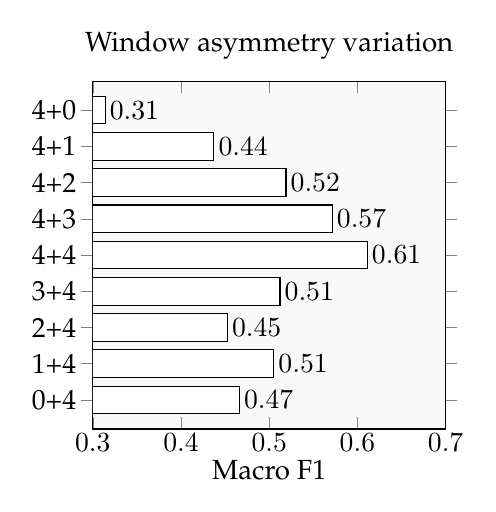
\begin{tikzpicture}
    \begin{axis}[
            title={Window asymmetry variation},
            xbar,
            axis background/.style={fill=gray!5},
            xmin=0.3,
            xmax=0.7,
            ytick=data,
            height=6cm,
            inner sep=1.5,
            xlabel={Macro F1},
            % height={ 1cm + ( 3.0 * 1cm ) },
            symbolic y coords={{0+4},{1+4},{2+4},{3+4},{4+4},{4+3},{4+2},{4+1},{4+0}},
            nodes near coords,
            nodes near coords align = {horizontal}
    ]
    \addplot[fill=white]
        coordinates {
        (0.4661,{0+4})(0.5052,{1+4})(0.4526,{2+4})(0.5122,{3+4})(0.6112,{4+4})(0.5715,{4+3})(0.5190,{4+2})(0.4373,{4+1})(0.3140,{4+0})
        };
    \end{axis}
    \end{tikzpicture}}
    \subfloat{
    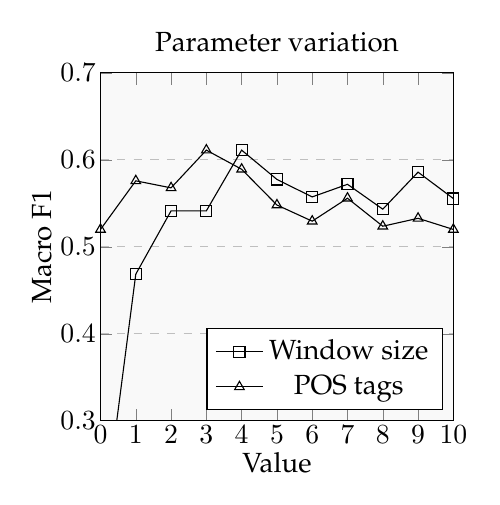
\begin{tikzpicture}
    \begin{axis}[
        title={Parameter variation},
        axis background/.style={fill=gray!5},
        ylabel={Macro F1},
        xlabel={Value},
        height=6cm,
        inner sep=1.5,
        xmin=0, xmax=10,
        ymin=0.3, ymax=0.7,
        xtick={0,1,2,3,4,5,6,7,8,9,10},
        ytick={0.3,0.4,0.5,0.6,0.7},
        legend pos=south east,
        ymajorgrids=true,
        grid style=dashed,
    ]
    \addplot[
        mark=square,
        ]
        coordinates {
        (0,0.1560)(1,0.4686)(2,0.5414)(3,0.5414)(4,0.6112)(5,0.5775)(6,0.5574)(7,0.5719)(8,0.5433)(9,0.5859)(10,0.5555)
        };
        \addlegendentry{Window size}

    \addplot[
        mark=triangle,
        ]
        coordinates {
        (0,0.5200)(1,0.5759)(2,0.5678)(3,0.6112)(4,0.5892)(5,0.5481)(6,0.5295)(7,0.5559)(8,0.5237)(9,0.5328)(10,0.5200)
        };

        \addlegendentry{POS tags}

    \end{axis}
    \end{tikzpicture}}

\end{minipage}

\end{posterbox}

%%%%%%%%%%%%%%%%%%%%%%%%%%%%%%%%%%%%%%%%%%%%%%%%%%%%%%%%%%%%%%%%%%%%%%%%%%%%%%

\begin{posterbox}[name=anaphora,column=1,below=cohesion]%
     {Results}
\begin{center}
    \hspace*{1cm}
    \begin{tabular*}{\columnwidth}{@{}rlllllll|l@{}}
          & ce  & cela & elle & elles & il  & ils & other & sum \\
    ce    & 165 & 3    & 0    & 1     & 8   & 1   & 6     & 184 \\
    cela  & 5   & 80   & 4    & 1     & 21  & 0   & 18    & 129 \\
    elle  & 7   & 10   & 22   & 2     & \textbf{22}  & 2   & 18    & 83  \\
    elles & 0   & 0    & 0    & 18    & 0   & \textbf{31}  & 3     & 51  \\
    il    & 11  & 7    & 9    & 0     & 64  & 1   & 12    & 104 \\
    ils   & 1   & 0    & 0    & 5     & 0   & 149 & 5     & 160 \\
    other & 10  & 12   & 9    & 1     & 9   & 15  & 338   & 394 \\
    \cline{1-8}
    sum   & 199 & 112  & 44   & 27    & 124 & 199 & \multicolumn{1}{l}{400}   & ~   \\
    \end{tabular*}
\end{center}
\begin{center}

    \begin{tabular}{llll}
          & \makebox[13mm][l]{Precision} & \makebox[13mm][l]{Recall}  & \makebox[13mm][l]{F1}      \\ \midrule
    ce    & 0.8291   & 0.8967 & 0.8616 \\
    cela  & 0.7143   & 0.6202 & 0.6639 \\
    elle  & 0.5000   & 0.2651 & 0.3465 \\
    elles & 0.6296   & 0.3333 & 0.4359 \\
    il    & 0.5161   & 0.6154 & 0.5614 \\
    ils   & 0.7487   & 0.9312 & 0.8301 \\
    other & 0.8450   & 0.8579 & 0.8514 \\
    \midrule
    \textbf{Macro} & 0.5816 & 0.5495 & 0.5530 \\
    \textbf{Micro} & 0.7213 & 0.7213 & 0.7213 \\
    \hline
    \end{tabular}

\end{center}

\begin{compactitem}
\item Results indicate that the model performs on par with similar models, while being easier to train.
\item There are some expected drops in performance for the less common classes heavily dependent on finding their antecedent.
\item A symmetric window size is beneficial, while we are not as sure of why this is the case.
\item Right context seems to be more important than left context, possibly due to the fact that pronouns in their role as subjects largely appears early in sentences.
\item There is potentially too little data for creating robust embeddings, except for in a few reoccurring circumstances.
\end{compactitem}


\end{posterbox}


\end{poster}%
\end{document}
